\section{Lasso}
   \subsection{模型介绍}
   Lasso在基础的线性回归模型的损失函数上,增加了L1正则项,假设有p个预测变量,此时Lasso损失函数如下:
   \begin{equation}
    \sum_{i=1}^n(y_i-\beta^Tx_i)^2+\lambda\sum_{j=1}^p|\beta_j|
   \end{equation}
   这里$\lambda$是超参数。
   
    \subsection{超参数$\lambda$选择}
    调用R语言glmnet包,实现Lasso Regression,将数据分成十份,计算不同超参数$\lambda$下交叉验证(Cross Validation)的误差,并选择最优的超参数,结果如图1所示
    \begin{figure}[htbp]
        \centering
        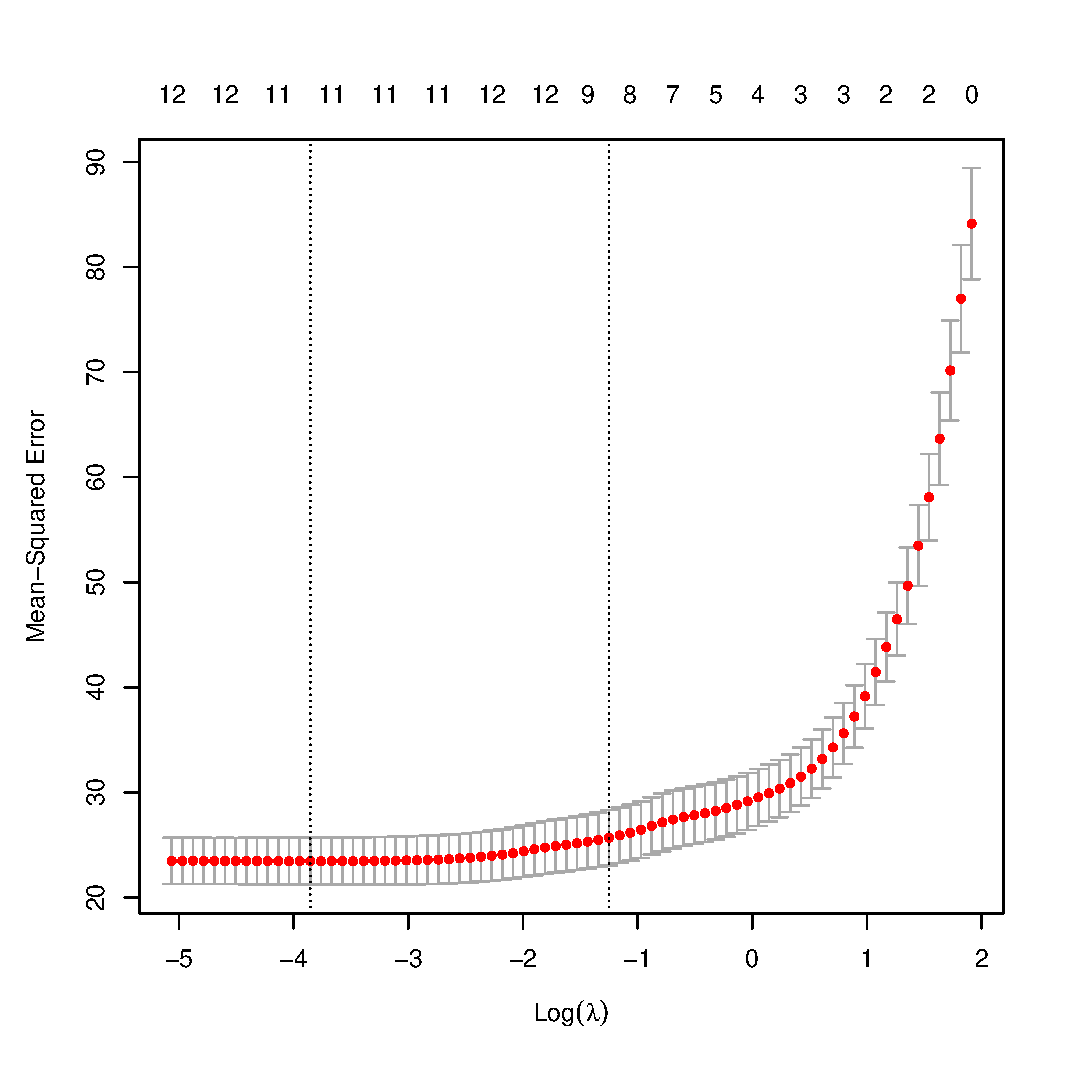
\includegraphics[width=0.6\textwidth]{lassocv.eps}
        \caption{Lasso Cross Validation}
    \end{figure}
    由结果可知,我们选取最小的均方误差对应的超参数系数,最优的$\lambda$取值约为0.021。
    \subsection{结果及分析}
    分别用glmnet包和自己编写的使用循环坐标下降法进行优化的代码在最优的$\lambda$取值下进行Lasso Regression,拟合得到的模型系数如表3所示
    \begin{table}[H]
        \centering
        \caption{自己编写与glmnet包用lasso估计系数的结果}
        \begin{tabular}{|c|c|c|c|c|c|c|c|c|c|c|c|c|c|c|}
        \hline
               & crim  & zn   & indus & chas & nox    & rm   & age  & dis   & rad  & tax   & ptratio & black & lstat & intercept \\ \hline
        glmnet & -0.10 & 0.04 & 0.00  & 2.69 & -16.57 & 3.85 & 0.00 & -1.42 & 0.26 & -0.01 & -0.93   & 0.01  & -0.52 & 34.91     \\ \hline
        ours   & -0.10 & 0.02 & -0.02 & 4.45 & -11.34 & 3.41 & 0.00 & -0.75 & 0.00 & 0.00  & 0.00    & 0.00  & -0.55 & 17.16     \\ \hline
        \end{tabular}
    \end{table}
    从表中我们可以看出,glmnet包的结果与我们的结果在各个项与房价的正负相关性上是相同的,但我们的结果将更多的系数压缩到0。存在这种差别的原因是lasso无法得到系数解析解,所以要采用别的计算方法,而我们优化计算系数的方式是循环坐标下降法,而R自带包计算系数的方法是最小角回归法,计算方法上最小角回归法更容易得到最优解。但两种方法的结果总体比较还是较为一致的。
    
    在glmnet的结果中,房价与crim犯罪率、nox氮氧化物浓度、dis到就业中心的距离、ptratio学生与教师比例、lstat人口数量呈负相关,与zn住宅用地比例、chas查尔斯河虚拟变量、rm每栋住宅的平均房间数、rad可达公路数、black黑人比例呈正相关,与indus、age两个变量无关,而这也与之前线性回归模型参数估计中,发现这两个变量的系数显著性检验并未通过的结果相一致。

    在我们的结果中。房价与犯罪率、indus商场面积、氮氧化物浓度、到就业中心的距离、人口数量呈负相关,与住宅用地比例、查尔斯河虚拟变量、每栋住宅的平均房间数呈正相关,与其余变量无关。

    以上结果都与常识相符,比如犯罪率与房价的负相关性。接下来我们比较超参数一致情况下,两种方式计算的MSE结果,两种代码的MSE如下表所示
    \begin{table}[H]
        \centering
        \caption{采用自己编写与glmnet包的系数计算的MSE比较}
        \begin{tabular}{|c|c|}
        \hline
               & MSE   \\ \hline
        glmnet & 21.92 \\ \hline
        ours   & 27.72 \\ \hline
        \end{tabular}
    \end{table}
    由结果可见,glmnet包训练的模型MSE更小,但是我们的循环坐标下降法本身选择的有效变量更少(系数非零的变量个数少),这样也会导致MSE增加,所以MSE不是一个很好的比较标准,但是采用最小角回归方法优化计算的lasso系数估计值更与线性回归的结果一致。
